\documentclass[12pt, letterpaper]{article}

% --- PAQUETES ---
\usepackage[utf8]{inputenc}
\usepackage[T1]{fontenc}
\usepackage[spanish]{babel}
\usepackage[left=2cm, right=2cm, top=2cm, bottom=2.5cm]{geometry}
\usepackage{enumitem}
\usepackage{amssymb}
\usepackage{tcolorbox}
% --- PAQUETE PARA FONDO ---
\usepackage{eso-pic}

% --- CONFIGURACIÓN DEL FONDO ---
\AddToShipoutPictureBG{%
	\AtPageLowerLeft{%
		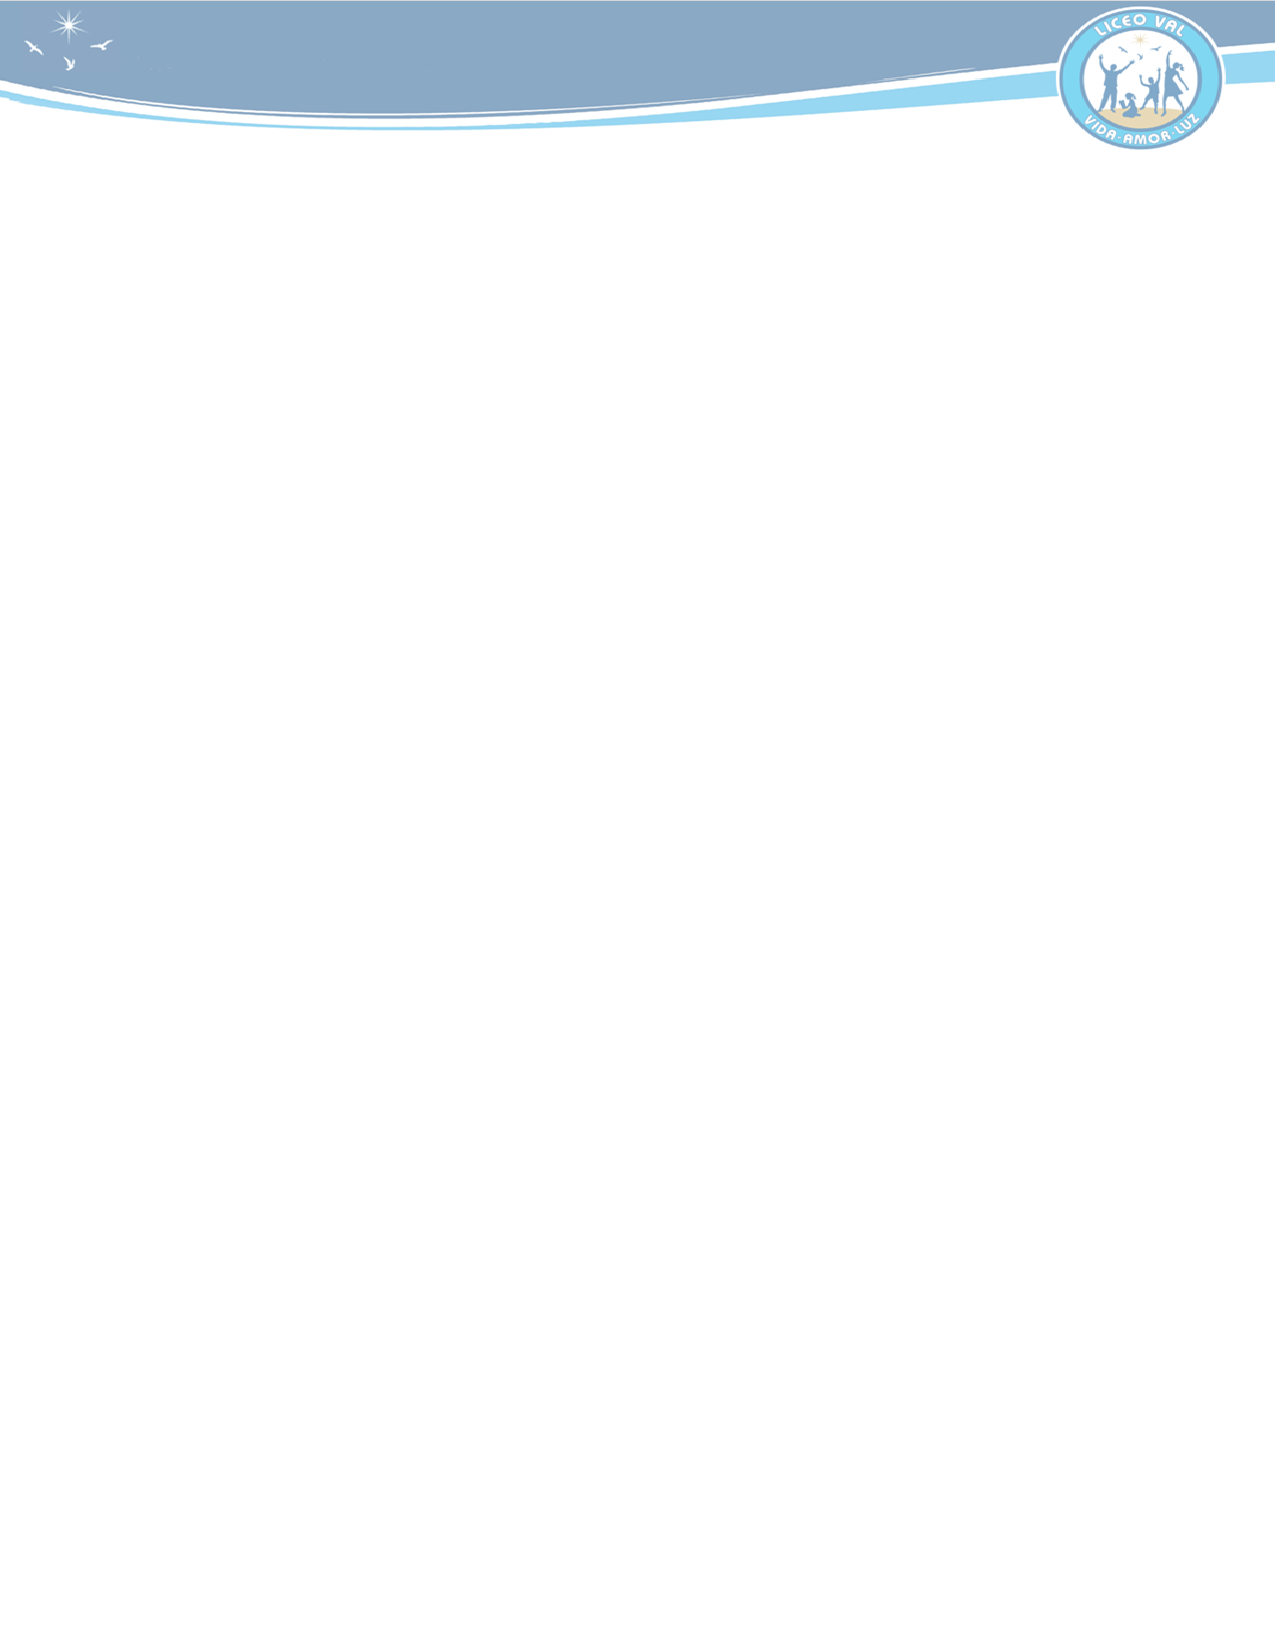
\includegraphics[width=\paperwidth,height=\paperheight,keepaspectratio=false]{../../FondoVAL.pdf}%
	}%
}

% --- FUENTE --- 
\usepackage{helvet} 
\renewcommand{\familydefault}{\sfdefault}

% --- COMANDO PARA CASILLAS DE RESPUESTA PEQUEÑAS --- 
\newcommand{\boxfill}[1][1.5cm]{\tcbox[on line, size=minimal, colframe=black, colback=white, boxrule=0.5pt, arc=1mm, boxsep=3pt, left=2pt, right=2pt, top=2pt, bottom=2pt]{\hspace*{#1}\vphantom{M}}}

\begin{document}
	
	% --- ENCABEZADO --- 
	\begin{center} 
		{\Large \textbf{LICEO V.A.L. (Vida, Amor, Luz)}}\\[0.2cm] 
		{\large \textbf{DEPARTAMENTO DE CIENCIAS BÁSICAS}}\\[0.2cm] 
		\textbf{Examen de CIENCIAS}\\[0.1cm] 
		%\textit{TAU 1: ¡Viajemos por dentro de la Tierra!} 
	\end{center}
	
	\vspace{0.3cm}
	\hfill \textbf{Código:} \textbf{L9-01}\\[0.1cm]
	\noindent \textbf{Nombre:} \underline{\hspace{8cm}} \hspace{1cm}\textbf{Fecha:} \underline{\hspace{3cm}}
	\vspace{0.8cm}
	
	
	% --- PUNTO 1 --- 
	\noindent \textbf{1.} Cuando el transbordador logra salir de la atmósfera y se sitúa en el vacío del espacio (a unos 2.500 kilómetros de altura), ¿cómo se ve nuestro planeta realmente, superando la ilusión óptica inicial? \hfill\textbf{(20\%)}
	
	\vspace{0.3cm} 
	\begin{itemize}[itemsep=0.4cm, label={}] 
		\item[ $\square$ ] Como un enorme plato de sopa plano. 
		\item[ $\square$ ] Como una hermosa esfera brillante y blanquiazul. 
		\item[ $\square$ ] Exactamente del mismo tamaño que la Luna. 
	\end{itemize}
	
	\vspace{0.5cm}
	
	% --- PUNTO 2 --- 
	\noindent \textbf{2.} La ciencia (geofísica) ha descubierto que el interior de nuestro planeta no es como lo imaginó Julio Verne. ¿Cuál de las siguientes capas de la Tierra está formada por materia \textbf{líquida} terriblemente caliente y pesada? \hfill\textbf{(20\%)}
	
	\vspace{0.3cm} 
	\begin{itemize}[itemsep=0.4cm, label={}] 
		\item[ $\square$ ] El Manto. 
		\item[ $\square$ ] El Núcleo interior.
		\item[ $\square$ ] El Núcleo exterior. 
	\end{itemize}
	
	\vspace{0.5cm}
	
	% --- PUNTO 3 --- 
	\noindent \textbf{3.} Lee cada afirmación sobre las dimensiones de la Tierra y marca con una \textbf{X} si es Verdadera (V) o Falsa (F): \hfill\textbf{(20\%)}
	
	\vspace{0.3cm} 
	\begin{itemize}[itemsep=0.6cm, label={}] 
		\item \textbf{A.} La distancia imaginaria desde la superficie hasta el centro exacto\ de la Tierra es de aproximadamente 6.400 kilómetros. \hfill  $\square$  V \quad  $\square$  F 
		
		\item \textbf{B.} La circunferencia (también llamada la ``cintura'') de la Tierra \ mide aproximadamente 10.000 kilómetros. \hfill  $\square$  V \quad  $\square$  F 
	\end{itemize}
	
	\newpage
	
	% --- PUNTO 4 --- 
	\noindent \textbf{4.} Imagina que decides darle la vuelta a la Tierra a caballo. La circunferencia (cintura) de la Tierra mide \textbf{40.000 kilómetros}. Si el caballo avanza a una velocidad de \textbf{10 km/h} y suponemos que solo viajas \textbf{10 horas al día}, ¿cuántos días te demorarías en completar el viaje? \hfill\textbf{(20\%)}
	
	\noindent \textit{Marca tu respuesta final:}
	\begin{itemize}[itemsep=0.4cm, label={}] 
		\item[ $\square$ ] 800 días (un poco más de dos años). 
		\item[ $\square$ ] 400 días (unos 13 meses, poco más de un año).
		\item[ $\square$ ] 40 días. 
	\end{itemize}
	
	\vspace{0.5cm}
	
	% --- PUNTO 5 --- 
	\noindent \textbf{5.} Lee cada afirmación sobre las profundidades oceánicas y marca con una \textbf{X} si es Verdadera (V) o Falsa (F): \hfill\textbf{(20\%)}
	
	\vspace{0.3cm} 
	\begin{itemize}[itemsep=0.6cm, label={}] 
		\item \textbf{A.} La palabra ``abisal'' viene del griego \textit{ábyssos} y significa ``sin fondo'',\ refiriéndose a las zonas marinas tan profundas que son totalmente oscuras. \hfill  $\square$  V \quad  $\square$  F 
		
		\item \textbf{B.} Cuando el submarino tocó el fondo de la Fosa de las Marianas,\ los biólogos comprobaron que allí no podía vivir ningún animal\ vertebrado debido a la inmensa presión. \hfill  $\square$  V \quad  $\square$  F 
	\end{itemize}
	
	
\end{document}